\documentclass{article}
\usepackage[utf8]{inputenc}
\usepackage[english]{babel}
\usepackage{amsthm}
\usepackage{amssymb}
\usepackage{mathtools}
\usepackage{enumerate}
\newcommand\tab[1][1cm]{\hspace*{#1}}
\usepackage{graphicx}
\usepackage[margin=0.75in]{geometry}

\author{Kevin Martin\\ CIS675 - Syracuse University}
\title{Homework 4}

\newtheorem*{claim}{Question}
\renewcommand\qedsymbol{$\blacksquare$} 
\begin{document}
\maketitle
\begin{enumerate}
  \item Question 1
    \begin{enumerate}
      \item The iterations of the maximum flow algorithm from node $S$ to node $T$:\\
        \begin{figure}[h]
              \centering
            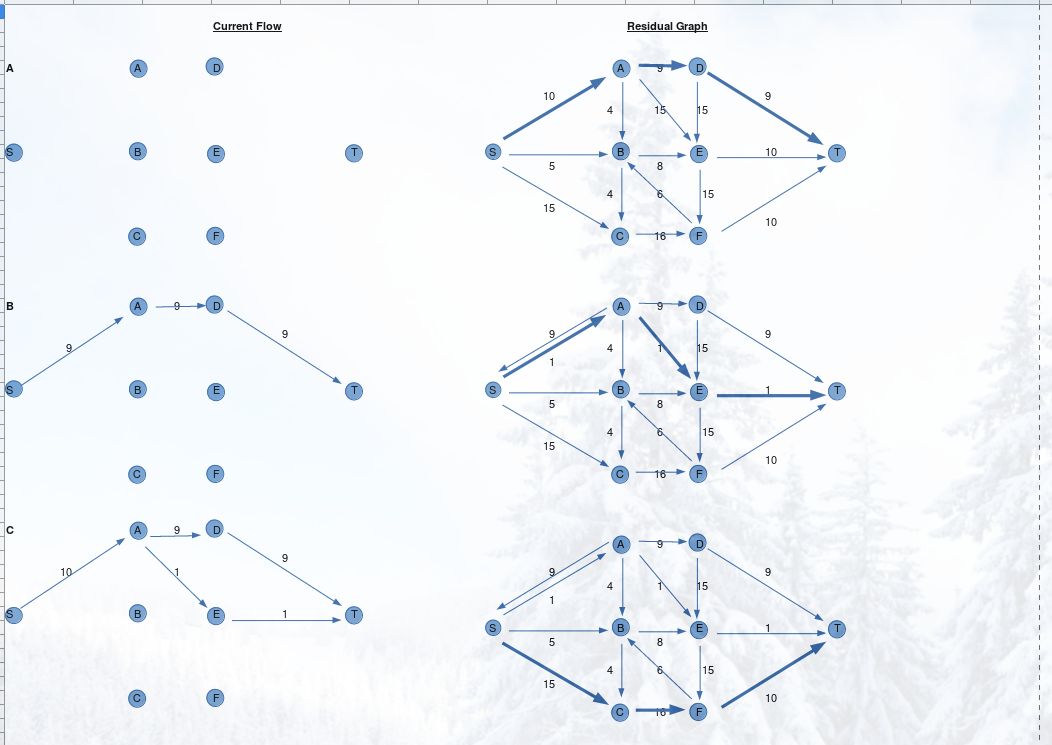
\includegraphics[scale=.36]{mincut1.png}
            \end{figure}

         
            \pagebreak
          \begin{figure}[h]
            \centering
          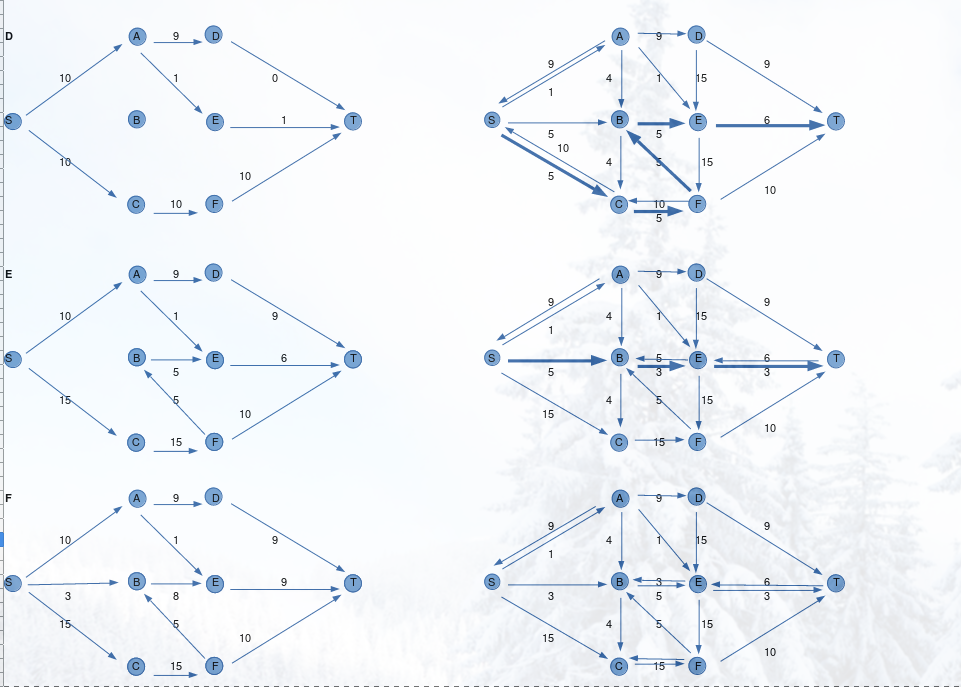
\includegraphics[scale=.36]{mincut2.png}
          \end{figure}
         \item The minimum cut:\\
        \begin{figure}[h]
            \centering
          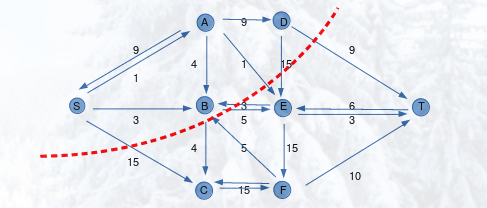
\includegraphics[scale=.36]{mincut3.png}
          \end{figure}

        \end{enumerate}


  \item Question 2
    For an undirected connected graph, $G=(V,E)$:\\
    \begin{enumerate}
    \item Algorithm for maximum spanning tree, negate the weights
      and apply Kruskal's algorithm:\\\\
      def maxSpan(G)\\
      \tab sortDescending(e) // sort all edges e in descending order\\
      \tab tree T = $\emptyset$\\
      \tab for i = 1 to n do // for all edges n\\
      \tab \tab (u,v) = $e_{i}$\\
      \tab \tab if setCheck(u) != setCheck(v) // no cycles\\
      \tab \tab \tab T = T $\cup$ {$e_{i}$} // merge sets containing u and v\\
      \tab \tab \tab if count(T) == n - 1 then\\
      \tab \tab \tab \tab break\\
      \tab return T

    \item The runtime is $O(E log V)$ where $E$ is the number of edges and $V$ is the number of
      vertices. We must use a comparision based algorithm to sort all the edges, which takes the majority
        of the running time. The rest of the operations can be done in constant $O(1)$ time., except
        for the find and union operations, witch take $O(Log V)$, which is still dominated by the
        sorting portion. The space complexity is $O(E + V)$ as we have to store all the edges and
        all the vertices to fully perform the algorithm.

    \end{enumerate}
      
  \item Question 3
    Given a convex polygon P with $n$ vertices in the plane:\\
    \begin{enumerate}
      \item Pseudocode of a dynamic programming algorithm to find triangulation of minimum cost of polygon P:\\\\
        def triangulate(V [], int n):\\
        \tab if (n$<$3) then\\
        \tab \tab return 0 // not a true polygon\\
        \tab matrix[n][n] \\
        \tab for (check = 0 : n) do \\
        \tab \tab for (i = 1, j = check, j $<$ n) do\\
        \tab \tab \tab if (j $<$ i + 2) then \\
        \tab \tab \tab \tab matrix[i][j] = 0\\
        \tab \tab \tab else\\
        \tab \tab \tab \tab matrix[i][j] = $\infty$\\
        \tab \tab \tab \tab for (k = i + 1, k $<$ j) do\\
        \tab \tab \tab \tab \tab temp = matrix[i][k] + matrix [k][j] + sum(V, i , j, k)\\
        \tab \tab \tab \tab \tab if (matrix[i][j] $>$ temp) then\\
        \tab \tab \tab \tab \tab matrix[i][j] \\
        \tab return matrix[0][n-1]\\

      \item The running time of this algorithm is an unfortunate $(On^3)$. This is because we must perform
        $n$ operations on a two dimensional matrix ($O(n^2)$). We must check the cost of each potential
        triangle, using the "sum" function, and store the results. Then we must compare those results to
        ensure our final result is the optimal (minimum) one. The space complexity for this algorithm is
        also large due to the matrix: $O(n^2)$ as we must complete a full $n$ x $n$ matrix.

    \end{enumerate}

  \item Question 4 Matching two gene strings using a socring sequence, accomedating for gaps:
    \begin{enumerate}
      \item Pseudocode of a dynamic programming algorithm to take in two strings and return highest
        scoring alignment of the two strings:\\\\
        def scoreCalc(A [], B[] )\\
        \tab score = 0\\
        \tab matrix[length(A) + 1][length(B) + 1] // store results\\
        \tab for i = 0 : length(A)\\
        \tab \tab matrix[i][0] = score * i\\
        \tab for j = 0 : length(B)\\
        \tab \tab matrix[0][j] = score * j\\
        \tab for i = 1 to length(A) + 1 do\\
        \tab \tab for j = 1 to length(B) + 1 do\\
        \tab \tab \tab match = matrix[i - 1][j - 1] + similarity(A[i], B[i])\\
        \tab \tab \tab delete = matrix[i - 1][j] + score\\
        \tab \tab \tab insert = matrix[i][j - 1] + score\\
        \tab \tab \tab matrix[i][j] = max(match, insert, delete)\\
        \tab return matrix[i][j] // this gives the max score \\\\

        def findAlignment(A [], B[])\\
        \tab alignA = 0\\
        \tab alignB = 0\\
        \tab i = length(A)\\
        \tab j = length(B)\\
        \tab while ( i $>$ 0 or j $>$ 0) do\\
        \tab \tab if (i $>$ 0 and j $>$ 0 and matrix[i][j] ==\\ 
        \tab \tab matrix[i - 1][j - 1] + similarity(A[i], B[i])) do\\
        \tab \tab \tab alignA = A[i] + alignA \\
        \tab \tab \tab alignB = B[j] + alignB \\
        \tab \tab \tab i -= 1 \\
        \tab \tab \tab j -= 1 \\
        \tab \tab else if (i$>$0 and matrix[i][j] == (matrix[i - 1][j] + score)) do\\
        \tab \tab \tab alignA = A[i] + alignA \\
        \tab \tab \tab alignB = "-" + alignB // gap, insert in B \\
        \tab \tab \tab i -= 1\\
        \tab \tab else \\
        \tab \tab \tab alignA = "-" + alignA // gap, insert in A \\
        \tab \tab \tab alignB = B[j] + alignB \\
        \tab \tab \tab j -= 1\\

      \item The running time is $O(n^2)$, assuming the input strings A and B are of the same length. If they
        were of different lengths $m$ and $n$, then the running time would be $O(mn)$. This is because each
        entry in the matrix must be calculated. The calculations are done in constant time but need to be 
        applied to the entire set of possible combinations. Similarly, the sapce complexity is also $(On^2)$,
        assuming the two input strings are equal (otherwise the space complexity would be $O(mn)$). This is
        because the algorithm fills the entire $n$ x $n$ matrix.


    \end{enumerate}

  \item Question 5
      \begin{enumerate}
        \item To represent the situation as a linear problem, we formulate as follows, letting 
          $x_{1}$ be regular drinks and $x_{2}$ be strong drink:\\\\
          \tab Objective function \tab max $2x_{1}+3x_{2}$  \\
          \tab Constraints \tab \tab $x_{1}+1.5x_{2} \leq 3000$  \\
          \tab \tab \tab \tab \tab $x_{1} + x_{2} \geq 300$\\
          \tab \tab \tab \tab \tab $2x_{1} \leq x_{2}$\\

        \item Graph of feasible region:
          \begin{figure}[h]
            \centering
        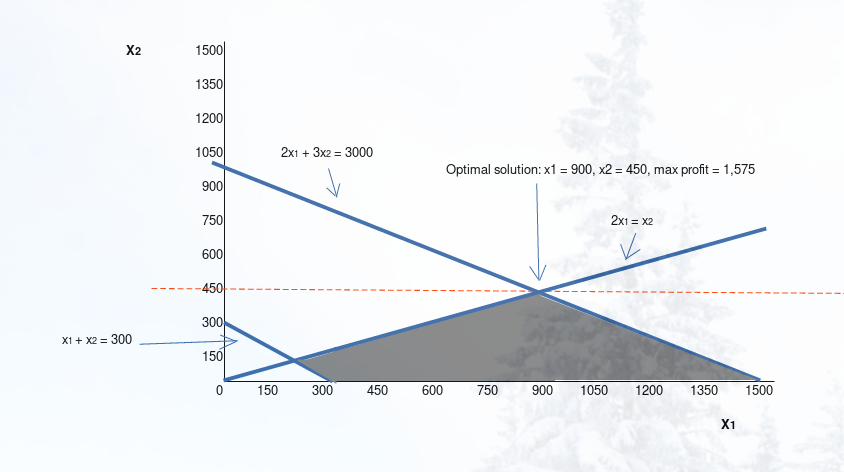
\includegraphics[scale=.55]{feasiblegraph4.png}
        \end{figure}
    
        \item The coordinates of all vertices of the feasible region are:\\
          (300, 0), (1500, 0), (900, 450), (200, 100)

        \item The optimal product mix to maximize daily profit is:\\
          900 regular drink at \$ 2 each and 450 strong drink at \$ 3 each, which 
          gives a total profit of \$1,575 per day.
          This is represented on the graph by the furthest out point on on the 
          feasible region, where the tangential dotted line intercepts the point
          (900, 450).

      \end{enumerate}

\end{enumerate}
\end{document}


